%-----------------------------------------------------------------------------
%
%               Statement for the VURM project
%
% Name:         statement.tex
%
% Purpose:      Short introduction to the project, goal definition and
%               deadlines listing for the project.
%
% Author:       Jonathan Stoppani
%               College of Engineering and Architecture Fribourg
%               jonathan@stoppani.name
%
% Created:      16 June 2011
%
%-----------------------------------------------------------------------------


\documentclass[10pt,authoryear]{sigplanconf} % add preprint option if needed

%--------------------------------------------------------------------------------

% Included and labeled graphics support
\usepackage{graphicx}

% Table support
\usepackage{tabularx}
\usepackage{booktabs}
\newcommand{\row}{\\\noalign{\smallskip}}

% Subfigures support
\usepackage[caption=false,font=footnotesize]{subfig}

% Manual footnotes counter for tables
\usepackage{fmtcount}

\usepackage{hyperref}
\hypersetup{
	% Removes frames from links
    pdfborder = {0 0 0}
}

% Autoref support for subfigures
\def\subfigureautorefname{Subfigure}

%--------------------------------------------------------------------------------

\begin{document}

%--------------------------------------------------------------------------------

% Copyright metadata
\copyrightyear{2011} 
\copyrightdata{Jonathan Stoppani}
%\authorpermission
\toappear{Permission to make digital or hard copies of all or part of this work for personal or classroom use is granted without fee provided that copies are not made or distributed for profit or commercial advantage and that copies bear this notice and the full citation on the first page. To copy otherwise, to republish, to post on servers or to redistribute to lists, requires prior specific permission.

\vspace{5pt}Copyright \copyright 2011, Jonathan Stoppani}

%--------------------------------------------------------------------------------

\title{VURM -- Project statement}
\subtitle{Virtual resources management on HPC clusters}

\authorinfo{Jonathan Stoppani}
           {College of Engineering and Architecture Fribourg}
           {jonathan.stoppani@edu.hefr.ch}



\maketitle

%--------------------------------------------------------------------------------

\begin{abstract}
Software deployment on HPC clusters is often subject to strict limitations with regard to software and hardware customization of the underlying platform. One possible approach to circumvent these restrictions is to virtualize the different hardware and software resources by interposing a dedicated layer between the running application and the host operating system.

The goal of this project is to enhance existing HPC resource management tools with special virtualization-oriented capabilities such as job submission to specially created virtual machines or runtime migration of virtual nodes to account for updated job priorities or for better performance exploitation.
\end{abstract}

\keywords
resource management, virtualization, HPC, slurm

%--------------------------------------------------------------------------------

\section{Introduction}

SLURM (Simple Linux Utility for Resource Management) is, as the name says, a resource manager for Linux based clusters of all sizes. Its job is to allocate resources to users requesting them by arbitrating possible contentions using a queue of pending work and to offer tools to start, execute and monitor work started on previously allocated resources.

To be able to support more esoteric system configurations than what allowed on common HPC clusters and to provide advanced job controlling capabilities (mainly pausing/resuming and migration), SLURM can be extended to support virtual clusters and virtual machines management.

A virtual cluster groups physical nodes togheter and can be thought of as a logical container for virtual machines. Such a cluster can be resized to account for workload changes and runtime job prioritization updates.

Virtual machines can be started inside a virtual cluster and run on a physical node. In low system load situations or for high priority jobs, each physical node hosts exactly one VM (\autoref{fig:low-load}). When additional or higher prioritized jobs are submitted to the system, these VMs can be migrated to already busy nodes to free up resources for the incoming jobs (\autoref{fig:migration} and \ref{fig:high-load}). The same procedure can be applied if some resources are released in order to increase the performances (\autoref{fig:restoration}).

\begin{figure}[h]
	\begin{center}
		\subfloat[Low load operation]{\label{fig:low-load}
		
\includegraphics[width=.48\columnwidth]{figures/statement/low-load}}
		\hfill
		\subfloat[Migration]{\label{fig:migration}
		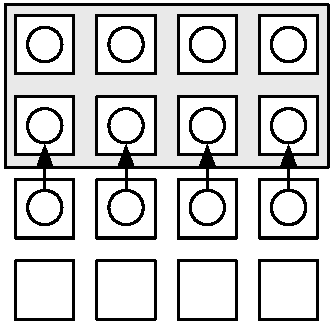
\includegraphics[width=.48\columnwidth]{figures/statement/migration}}
		
		\subfloat[High load operation]{\label{fig:high-load}
		
\includegraphics[width=.48\columnwidth]{figures/statement/high-load}}
		\hfill
		\subfloat[Restoration]{\label{fig:restoration}
		                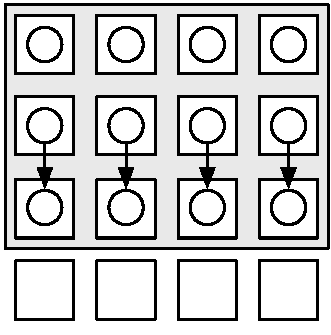
\includegraphics[width=.48\columnwidth]{figures/statement/migration-back}}
	\end{center}
	\caption{VMs migration process to allocate resources for an higher prioritized job in its different states: before, during allocation, while running both jobs and after. (Squares represent physical nodes, circles represent VMs and darker rectangles are virtual clusters.)}
	\label{fig:migration-process}
\end{figure}

%--------------------------------------------------------------------------------

\section{Goals}

The ultimate goal of this project is to add support for the virtual resources management capabilities described above to SLURM. These capabilities can either be provided as plugins or by directly modifying the source tree.

To reach this objective, different partial goals have to be attained. The following list summarizes them:

\begin{enumerate}
\item Adding support for starting and stopping virtual clusters in SLURM with the newly-created virtual clusters attaching to the existing SLURM instance and on which regular jobs can be launched.

This will require adding support for the libvirt or related virtualization management libraries to SLURM.

\item Adding support for controlling the pausing and migration of virtual machines to SLURM so that more sophisticated resource allocation decisions can be made (e.g. migrating multiple virtual machines of a virtual cluster onto a single physical node) as new information (e.g. new jobs) become available.

\item Implementing simple resource allocation strategies based on the existing job scheduling techniques to demonstrate the capabilities added to SLURM, KVM, and Palacios in (1) and (2) above.
\end{enumerate}

%--------------------------------------------------------------------------------

\section{Deadlines}

The deadlines for the project are resumed in the \autoref{tbl:deadlines}. For more detailed information about the content of each deliverable or milestone, refer to the planning document.

\addtocounter{footnote}{1}
\footnotetext[\value{footnote}]{All dates refer to 2011}

\addtocounter{footnote}{1}
\footnotetext[\value{footnote}]{M=Milestone, D=Deliverable}
\addtocounter{footnote}{-1}

\begin{table}[ht]
\begin{tabularx}{\columnwidth}{ l c X }
\toprule\noalign{\smallskip}
Date$^{\decimal{footnote}}$ \addtocounter{footnote}{1}& Type$^{\decimal{footnote}}$ & Asset
\row\hline\hline\noalign{\smallskip}\noalign{\smallskip}
Jun. 6 & M & Project start 
\row
Jun. 20 & D & Project statement
\row
Jun. 20 & D & Planning
\row
Jul. 1 & M & Dynamic partitions
\row
Jul. 8 & M & Virtual clusters
\row
Jul. 15 & M & Virtual cluster pausing/resuming
\row
Jul. 15 & D & Project summary (EN/DE)
\row
Jul. 22 & M & Virtual cluster resizing
\row
Jul. 29 & M & Migration strategy
\row
Aug. 19 & D & Final presentation
\row
Aug. 19 & D & Final report
\row
Aug. 19 & D & Project sources and documentation
\row
Aug. 19 & M & Project end
\row
Sep. 7 & M & Oral defense
\row
Sep. 7 & D & Project poster
\row
\bottomrule
\end{tabularx}

\nocaptionrule\caption{Deadlines for the project.}
\label{tbl:deadlines}

\end{table}

%--------------------------------------------------------------------------------

\appendix
\section{Context}

This work is carried out at Scalable Systems Lab (SSL) of the Computer Science department of the University of New Mexico, USA (UNM) during Summer 2011.

The project will be based on SLURM (Simple Linux Utility for Resource Management) as underlying layer for resources management and two different virtual machine monitors: KVM and Palacios. KVM (Kernel-based Virtual Machine) is a general purpose virtual machine monitor which integrates directly into the Linux kernel, while Palacios is an HPC-oriented hypervisor designed to be embedded into a range of different host operating systems, including lightweight Linux kernel variants and thus potentially including the Cray Linux Environment.

%--------------------------------------------------------------------------------

\section{Experts and Supervisors}

Prof. Peter Kropf, Head of the Distributed Computing Group and Dean of the Faculty of Science of the University of Neuchatel, Switzerland covers the role of expert.

Prof. Patrick G. Bridges, associate professor at the University of New Mexico is supervising the project locally.

Prof. Pierre Kuonen, Head of the GRID and Cloud Computing Group, and Prof. Fran\c{c}ois Kilchoer, Dean of the Computer Science Department, both of the College of Engineering and Architecture Fribourg, are supervising the project from Switzerland.

%--------------------------------------------------------------------------------

\section{Useful resources}

\begin{itemize}
\item \url{https://computing.llnl.gov/linux/slurm/}

Official web site of the SLURM project website. Sources, admin/user documentation, papers as well as a \emph{configuration tool} can be found on there.

\item \url{http://www.linux-kvm.org/}

Web site of the KVM (Kernel-based Virtual Machine) project. A special page describing VM migration using KVM is available.

\item \url{http://www.v3vee.org/palacios/}

Official web site of the Palacios VMM project, developed as part of the V3VEE project. Access to news, documentation and source code is available.

\end{itemize}

%--------------------------------------------------------------------------------

%\acks

%Acknowledgments, if needed.

%--------------------------------------------------------------------------------

\bibliographystyle{abbrvnat}

%\begin{thebibliography}{}
%\softraggedright

%\bibitem[Smith et~al.(2009)Smith, Jones]{kvm}
%Text...

%\end{thebibliography}

\end{document}
